%===================================== CHAP 3 =================================

\chapter{Basic Theory}

\section{Artificial Neural Networks}

An implementation of the aforementioned feed-forward back-propagation (FFBP) for learning, can be outlined as follows:
\\
Consider a set of nodes of (artificial) neurons. Each node is connected to a subset of other nodes, and together they form a network. Topologically speaking, is is common in traditional approaches to simply construct a given number of layers with each node being connected to one or more nodes in the former and next layer of the network (see figure \ref{fig:three_layer_ann}), with distinct weights $\omega$ for each connection. In such an approach, the first layer is the input layer, whereas the last layer is the output layer. Data is then presented to the nodes of the input layer, propagated through the hidden layers by using a transfer function and the network weights, before finally arriving at the output nodes, which may represent any functional mapping such as classification, or action selection. Once the input has been propagated throughout the network (fed forward), the obtained output is matched with a desired output, and an error signal is generated (this can be regarded as the difference between the desired and current output). The error signal is then propagated backwards, the weights being updated to adjust for the error. Note that a learning rate constant, $\alpha$, is usually used to restrain the rate of adjustment in order for a solution to converge.
The transfer function is a function of a node's input, transforming its external input to internal activity. In a sense, the transfer function can be regarded as a crude mathematical approximation to a neuron's internal dynamics, usually providing boundaries for a neuron's possible activation values (representing its membrane potential). Weights may be any real valued numbers, but are usually constrained to a certain interval, for instance the interval of [-1, 1]. Some traditional approaches use only binary or tertiary weights, consisting of a set of the weights of -1, 0, or 1.
\\
\\

Mathematically speaking, ANNs may be formalised as the following;
\\
a network consists of a set $S$ of $N$ nodes. Furthermore, for every node $i\in S$: $i$ may be connected to a node $j \in S$.
\\
For every such connection, there exists a weight, $\omega_{i,j} \in \Re$, the sub-script denoting a connection weight from node $i$ to node $j$.
\\
A transfer function $f$ is a function $f(\theta)$ of a neuron's total input, $\theta$. A commonly used transfer function is the sigmoid transfer function, simply being 
\begin{equation}\label{sigmoid}
    f(\theta) = \frac{1}{1+e^{-\theta}}
\end{equation}

Neuronal activation $u_j$ of a node $j$ ca be formalised as follows,

\begin{equation}\label{input}
    \theta_j = \sum_{i\in M} u_i \omega_{i,j}
\end{equation}
\begin{equation}\label{activation}
    u_j = f(\theta_j)
\end{equation}
where $M$ is the set of all nodes that are connected to neuron $j$, $M \in S$, and $u_i$ is the activation value of node $i$. This is the principle which is used during the feed-forward phase in an FFBP ANN. In other words, the presented input is propagated throughout the network by calculating activation values for all nodes in the input layer, which then flows through the rest of the nodes in the network in the same manner, until finally arriving at the output nodes.

\begin{figure}
\centering
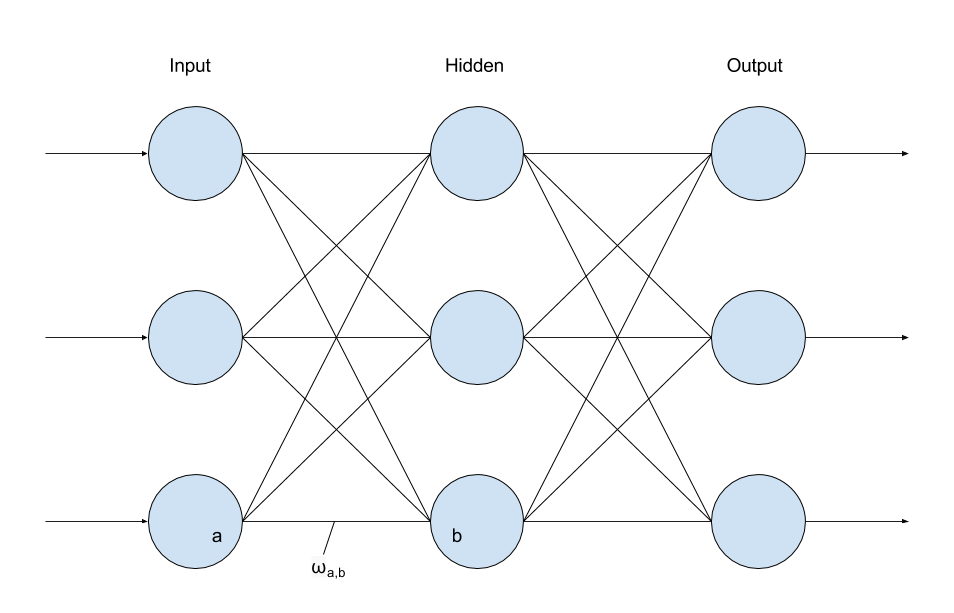
\includegraphics[width=10cm]{fig/three_layers_weight}
\caption{Illustrating a simple three-layer neural network with information flowing from left to right. Every line from one node to another represents a weight $\omega_{i,j}$ connecting two nodes. Note that all nodes are fully connected to each node of the next layer in this example.}
\label{fig:three_layer_ann}
\end{figure}


% =====================================================
\subsection{The Back-propagate Algorithm}\label{BP}

One way of updating the weights in an ANN is by using the back-propagate (BP) algorithm. It is a fairly straight-forward algorithm for searching for optimal weights in an ANN for a particular set of input-output patterns, by minimizing an error-signal which is back-propagated throughout the network. As the generation of an error signal requires an input pattern to be fed forward throughout a network, these two steps are commonly referred to together as feed-forward back-propagation (FFBP). Note, however, that the algorithm does not guarantee convergence towards a global optimum, as it is a gradient-based method, traversing the weight space for a neural network. See figure \ref{fig:steepest_descent} for an illustration of this. An analogy is simulated annealing, which runs the risk of being stuck in a local optimum. However, with just enough 'jiggle', the algorithm may manage to find a better solution, continuing the descent towards a more optimal solution.

Mathematically the back-propagate algorithm requires us to be able to generate a difference for each weight $\omega \in \Omega$, where $\Omega$ is the weight space for the network. Arriving at a given output for a given FFBP ANN through feed-forward propagation using the equations \eqref{sigmoid}, \eqref{input}, \eqref{activation}, we may express the squared error as,

\begin{equation}
    \textbf{E} = \frac{(\textbf{d} - \textbf{o})^2}{2},
\end{equation}
where $\textbf{d}$ is the desired output vector for all output nodes. Dividing by two to account for using two data points in finding the squared error.

This may then be used to calculate a gradient that we may use to update every weight between the output layer and the preceding layer in the ANN,

\begin{equation}\label{weight_update}
    \omega_{t+1}^{i,j} = \omega_{t}^{i,j} + \Delta \omega_{t}^{i,j},
\end{equation}

As we wish to perform a weight change in the direction of minimising the error loss function $\textbf{E}$, we use the partial derivative of $\textbf{E}$ w.r.t. the weight $\omega_{i,j}$,

\begin{equation}
    \Delta \omega_{i,j} = -\alpha \frac{\partial \textbf{E}}{\partial \omega_{i,j}},
\end{equation}

where $\alpha$ is a learning rate parameter. Note that we drop the sub-script denoting time for the sake of convenience.
The negative is used in order to adjust for the error. Despite the fact that BP does not guarantee convergence towards the global optimum (here minimum), it can be shown that for a sufficiently fine-grained step-parameter (i.e. learning rate), convergence towards a local optimum can be guaranteed. This is due to the nature of the search space, which is continuous and differentiable, but may contain ridges and local minimums in terms of the squared error, $\textbf{E}$. However, the smaller the learning rate $\alpha$, the slower the convergence. Another aspect is that for too low an $\alpha$, the gradient's "reach" will also decrease, making it more prone to small stationary points in the weight space. In other words, we want to try and attain a learning rate parameter which will converge fairly quickly towards an optimum. An analogy is that if $\alpha$ is too large, we are at the edge of chaos, resulting in divergence when using gradient descent in weight space. See figure \ref{fig:steepest_descent} for an illustration of this.

The following derivation is based primarily on the derivation of \cite{Rumelhart1986}, as well as on that of \cite{Russell2009}.
Using the chain rule, we may formally derive $\Delta \omega$ the following way,

\begin{equation}
    \frac{\partial \textbf{E}}{\partial \omega_{i,j}} = \frac{\partial \textbf{E}}{\partial u_j}
    \frac{u_j}{\theta_{j}}
    \frac{\theta_{j}}{\omega_{i,j}},
\end{equation}

the partial derivative w.r.t. the weight between nodes $i$ and $j$ will be cancelled out for all nodes other than $j$. Formally,

\begin{center}
\begin{math}
    \frac{\partial \theta_j}{\partial \omega_{i,j}} = \frac{\partial}{\partial \omega_{i,j}}(\sum_{k \in M}{} \omega_{k,j}o_k),
    \frac{\partial \omega_{k,j}o_k}{\partial \omega_{i,j} = 0 : k \neq i}
    \implies
\end{math}
\end{center}

\begin{equation}\label{delta_theta}
    \frac{\partial \theta_j}{\partial \omega_{i,j}} = u_i.
\end{equation}

\begin{equation}
    \frac{\partial u_j}{\partial \theta_j} = \frac{\partial}{\partial \theta_j} f(\theta_j) = f(\theta_j)(1-f(\theta_j))
\end{equation}

\begin{equation}
    \frac{\partial \textbf{E}}{\partial u_j} = \sum_{l \in L}(\frac{\partial \textbf{E}}{\partial \theta_l} 
    \frac{\partial \theta_l}{\partial u_j})
    = \sum_{l \in L}(\frac{\partial \textbf{E}}{\partial u_l} \frac{\partial u_l}{\partial \theta_l} \omega_{j,l}),
\end{equation}
where $L$ is all nodes to which node $j$ is connected - i.e. the set of nodes with \textit{outgoing} links from $j$. From this it can be seen that when $l$ is an output node,

\begin{center}
\begin{math}
    \frac{\partial \textbf{E}}{\partial u_l} \frac{\partial u_l}{\partial \theta_l} \omega_{j,l} = 
    u_l (u_l - d_l) \omega_{j,l},
\end{math}
\end{center}
Making it possible to obtain the partial derivatives recursively by starting at the output layer and surprisingly back-propagating the values into the partial derivatives for $\textbf{E}$ for every weight $\omega_{i,j}$.

In other words, the weight change update in a given layer accounts for the weight change updates of the preceding layers too. Formally,

\begin{equation}\label{recursive_derivative_error_activation_input}
    \frac{\partial \textbf{E}}{\partial u_j}\frac{\partial u_j}{\partial \theta_j} = 
    (\sum_{l \in L}\frac{\textbf{E}}{\partial u_l}\frac{\partial u_l}{\partial \theta_l}) f(\theta_j)(1-f(\theta_j).
\end{equation}

\begin{figure}
\centering
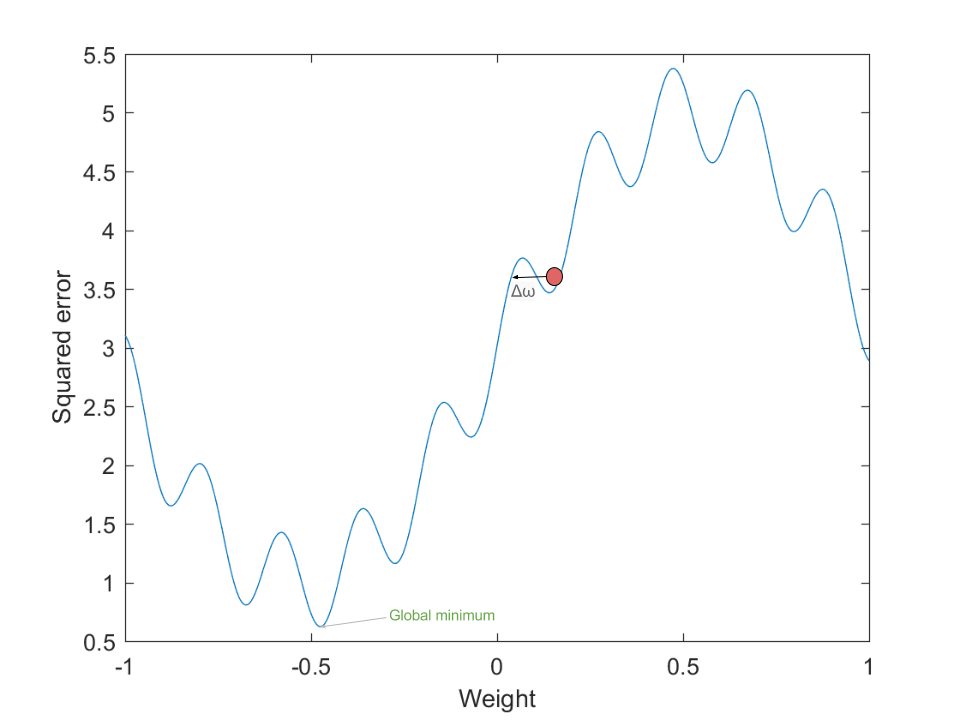
\includegraphics[width=10cm]{fig/error_landscape_with_ball.png}
\caption{Illustrating the error-landscape formed by finding the weights in an ANN that minimize the error. When traversing the landscape formed by $\textbf{E}$, local minimums may be encountered (in between ridges). An analogy which is often used in illustrating this is a ball rolling down the hill because of the kinetic energy imposed on it. In this analogy $\alpha$ would be constraining the work of gravity, resulting in smaller or larger velocities, i.e. step sizes $\Delta \omega$ for each iteration of the algorithm.
Too small an acceleration may result in the ball stopping when hitting a small ridge. In the event of this being a local minimum, we would of course prefer for the ball to have enough kinetic energy to traverse the ridge and fall into a lower valley. Therefore, just enough acceleration to traverse the local minimums is preferable. However, using too high an acceleration, the ball might not settle into any attractor, possibly the weights will even diverge, the ball being launched into outer space, settling its fate to never again return to the hillside.}
\label{fig:steepest_descent}
\end{figure}

% ===============================================================================
\subsection{A Trivial Example}

Consider an example network where the input layer consists of three nodes. A trivial case is where the input nodes are all binary, for instance symbolising a traffic light with three states; either red, yellow, or green. Thus the input to the network would either be {1, 0, 0}, {0, 1, 0}, or {0, 0, 1}, respectively. These nodes could be connected to nodes in a so called hidden layer, a layer which is neither an input nor an output layer of nodes, which again would be connected to an output layer. For this trivial example, consider that these three nodes are directly connected to the output layer, consisting of one node, which corresponds to an action: Walk or wait. It can fairly easily be seen that a successful action selection can be extracted for weights of {1, -1, -1}, if we interpret the output as walk for positive values, and wait for negative values of output. The transfer function is in this case simply the same as a node's total input $\theta_j$.

% ====================================
\subsection{Back-propagation Through Time}

The algorithm of section \ref{BP} may be extended by taking into account the $k$ last time-steps of training in the network. Implementations may vary, the key here being a time-dependence. By introducing a measure which averages over the former weights, it turns out that convergence may be faster than when only using BP (as opposed to here BPTT). An alternative approach is to include $k$, or all previous weights, discounting the impact each former weight has exponentially as a function of time.

\begin{center}
\begin{math}
    \omega_{t+1} = \sum_{i=0}^{k}\gamma^i \omega_{t-i},
    \gamma \in (0, 1)
\end{math}
\end{center}

% =================================================================================================
\section{The Dual-network Memory Architecture}

\cite{McClelland1995} proposes in their seminal paper a dual-network memory model which largely ameliorates the problem of catastrophic forgetting in ANNs, outperforming other algorithms of the time by far. Further work on this model is fairly limited, and we regard one of the latest papers on the dual-network memory architecture with the aim of further extending it. \cite{Hattori2010} proposes a model which fundamentally differs from the former implementations of \cite{French1997} and \cite{Ans1997} in that the hippocampal module is constituted by a chaotic neural network. Note that the phrases of hippocampal and neocortical networks should only be considered as borrowed terms for symbolising the parts of the model, as the networks are only very loosely coupled to it - the approach outlined here is only inspired by the workings of the brain.

\subsection{The Neocortical Network}

\cite{Hattori2010} trains the neocortical module using pseudopatterns. A pseudopattern is a pattern representing the weighting and internal dynamics of a network. In his paper, \cite{Hattori2010} looks at two types of pseudopatterns, which he refers to as type I and II. Type I is constructed in a very simple way: A random input is presented to the neocortical network, and the output is retrieved. This is then stored as an input-output pattern, called a pseudopattern of type I.

Pseudopatterns of type II are constructed in a slightly different manner, the approach being as follows:

\begin{enumerate}
\item Retrieve an extracted pattern from the hippocampal network.
\item For each element of the pattern, reverse is with a probability $p_r$.
\item Present the pattern to the neocortical network, and store the retrieved input-output pair (pseudopattern II) in a set.
\item Repeat step 2. and 3. until a certain number of pseudopatterns of type II are obtained.
\end{enumerate}
Performing steps 1.-4. above results in a set of pseudopatterns of type II.

After pseudopatterns have been obtained, the neocortical network is simply trained on them by using FFBP, i.e. standard gradient descent in weight space as outlined in \ref{BP}. Note that due to the nature of the pseudopatterns, old memories are actually interleaved with old. This may be seen by considering that pseudopattern I is in fact the output obtained by presenting a random input to the network, the output reflecting a compressed version of the network weights at the time. When the network is trained on the pseudopattern along with a hippocampal pseudopattern, BP attempts to minimise the error between the old configuration of weights and the new hippocampal pseudopattern. Thus interleaving the old representation of memories with the new memory. In fact, \cite{Hattori2014} uses the exact same type of mechanisms for memory consolidation to the neocortical network.
Similarly, for a set of pseudopatterns II, as elements are reversed in the hippocampal pseudopattern, the resulting pseudopatterns II reflect both the network configuration (weights) and the novel hippocampal pseudopattern. This is a more explicit type of interleaving, where a new pattern which is to be learned is slightly randomized, creating a set of patterns which will reflect both the new memory as well as the old.

Memory recall in the neocortical network may be performed by presenting input patterns to the neocortical network and obtaining the resulting output from the network. Note that as outlined above, the neocortical network only learns the pseudopatterns that are extracted by the hippocampal network. Therefore, some success criteria such as perfect recall depends strongly on the perfect extraction rate of the hippocampal network (i.e. when every part of the pattern has been successfully learned).

% ====================================
\subsection{The Hippocampal Network}
\subsubsection{\cite{Hattori2010}}
\begin{figure}
\centering
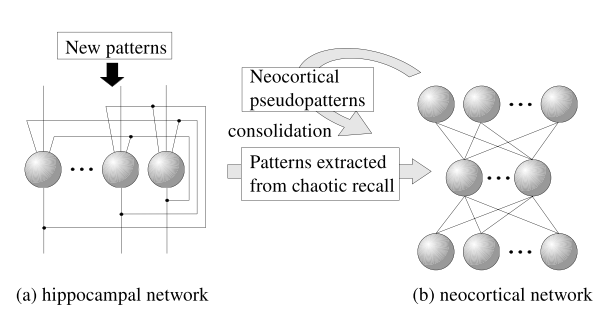
\includegraphics[width=10cm]{fig/hattori2010_model_structure}
\caption{An illustration from the paper of \cite{Hattori2010} of the proposed model. (a) represents the hippocampal module, whereas (b) represents the neocortical module. Note that the hippocampal module implements a Hopfield network, from which seemingly chaotic behaviour emerges when combined with the neuronal dynamics.}
\label{fig:hattori2010_model_structure}
\end{figure}

As can be seen from figure \ref{fig:hattori2010_model_structure}, \cite{Hattori2010} proposes a model in which the hippocampal (HPC) module is a single layer Hopfield network. However, the HPC module is not trained using gradient descent, but rather with Hebbian learning, which may be summarised as; fire together, wire together. Using Hebbian learning leads to faster convergence when compared with SGD (\cite{Hattori2010}). Adopting \cite{Hattori2010}'s notation, the model may be formally outlined as follows, beginning with the equation for Hebbian learning;

\begin{equation}\label{hattori_hebbian_learning}
    \omega_{i,j}(t+1) = \gamma \omega_{i,j}(t) + x_i^{(k)} x_j^{(k)},
\end{equation}

where $\omega_{i,j}(t+1)$ is the weight between neurons $i$ and $j$ for time step $t+1$, $\gamma$ is a constant forgetting factor ($\gamma \in (0, 1)$), and $\textbf{x}^{(k)} = (x_1^{(k)}, x_2^{(k)}, ..., x_N^{(k)})$ is the $k$-th pattern that we want the network to learn. Note that $\textbf{x}^{(k)} \in \{-1,1\}^N$, which constrains $x_i^{(k)} x_j^{(k)} \in [-1,1] \implies \omega_{i,j} \in [-1-\gamma, 1+\gamma]$. $N$ is the number of nodes in the input patterns.

Further, \cite{Hattori2010} outlines the neuronal dynamics as follows;

\begin{equation}\label{hattori_next_output}
    u_j(t+1) = f\{\eta_j (t+1) + \zeta_j(t+1)\}
\end{equation}

\begin{equation}\label{hattori_former_inputs}
    \eta_j(t+1) = k_m \eta_j(t) + \sum_{i=1}^{N} \omega_{i,j} u_i(t)
\end{equation}

\begin{equation}\label{hattori_zeta}
    \zeta_j(t+1) = k_r \zeta_j(t) - \alpha u_j(t) + a_j
\end{equation}

Adopted to our notation, $u_j$ is neuron $j$'s activation value, where the value for the next time step is determined by two functions, namely $\eta(t+1)$ and $\zeta(t+1)$. Equation \ref{hattori_former_inputs} takes into account its former input values through $\eta_j(t)$ for the current time step, in addition to summing over the inputs of its incoming synaptic connections. Equation \ref{hattori_zeta} includes a relationship to the neurons' previous activation values. Note that an external input parameter $a_j$ is also included in $\zeta_j(t+1)$, and that both equations \ref{hattori_former_inputs} and \ref{hattori_zeta} have damping factors of refractoriness $k_m$ and $k_r$, respectively, discontinuing the impact of former function-values exponentially relative to the temporal difference. $f(u)$ is the sigmoid function as defined in equation \ref{sigmoid}, note however that a steepness parameter $\epsilon$ is also included, $\theta$ being divided by $\epsilon$ such that

\begin{center}
\begin{math}
    f(\theta) = \frac{1}{1 + e^{\frac{-\theta}{\epsilon}}}
\end{math}
\end{center}

% ====================================
\subsubsection{\cite{Hattori2014}}
\cite{Hattori2014} proposes a more biologically inspired dual-network memory model, based on and outperforming the model outlined above based on several experiments. In the novel model, \cite{Hattori2014} proposes a rather drastic architectural change in the hippocampal network, the neocortical module remaining the same. The hippocampal module is made out of five layers, the three middle layers being inspired by different parts of the hippocampus; namely the entorhinal cortex (EC), dentate gyrus (DG), and CA3, the first and last layer being the input and output layers. See figure \ref{fig:hattori_2014_model} for the topological structure of the novel model of \cite{Hattori2014}.

\begin{figure}
\centering
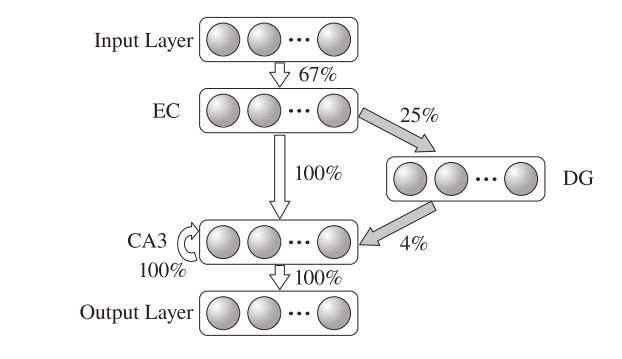
\includegraphics[width=10cm]{fig/hattori2014_hpc_module}
\caption{This figure by \cite{Hattori2014} illustrates his proposed dual-network memory model. Note that the EC is connected to both CA3 and DG, which in turn is also connected to CA3. The gray arrows are connections which are only used during training. Furthermore, CA3 is fully connected both recurrently as well as to the output layer. As EC is connected somewhat sparsely to the DG, and DG is very sparsely connected to CA3, this may constitute a form of compression mechanism as seen in auto-encoders. It is also worth noting that this poses a time-delay from when a certain input has been directly presented from the EC to CA3 until the possibly compressed input arrives from the DG. This may further constitute mechanisms similar to those of operating at multiple timescales, as well as mechanisms for abstraction.}
\label{fig:hattori_2014_model}
\end{figure}

It is worth mentioning that a slightly different transfer function is used by \cite{Hattori2014}. Namely,

\begin{center}
    $f(\theta) = tanh(\frac{\theta}{\epsilon})$,
\end{center}
where $\epsilon$ still is a steepness parameter.

Hebbian learning is still used as in equation \ref{hattori_hebbian_learning} for the CA3-layer and the CA3 to output-layer, relative to its former output;

\begin{center}
\begin{math}
    \omega_{i,j}(t+1) = \gamma \omega_{i,j}(t) + u_i u_j
\end{math}
\end{center}

However, between the EC and DG, EC and CA3, and DG and CA3 parts, Oja's rule is used (\cite{Hertz1991}, cited in \cite{Hattori2014}). Oja's learning rule is a modified type of Hebbian learning, restricting the weight space (to prevent divergence as a result of the chaotic behaviour) (\cite{}). It may be formally outlined as follows,

\begin{equation}\label{ojas_rule}
    \omega_{i,j} = \omega_{i,j}(t) + \lambda u_j (u_i - u_j \omega_{i,j}(t)),
\end{equation}
where $\lambda$ is the learning rate for the Oja neurons. Note that the input and output layer neurons are bipolar ($\pm 1$), whereas the other neurons are binary. Every region is trained by a k-winner-takes-all (kWTA) approach, in which a fixed number of the $k$ most active neurons' activation values are propagated throughout the neurons' synapses. Neuronal activity is determined by firing frequency. Interestingly, Hattori notes that the non-linear separation of kWTA seems to be far more powerful than that of non-linear transfer functions. Furthermore, he notes that non-linear transfer functions may actually reduce the performance of kWTA.

One of the final keys to attaining a successful dual-network memory model introduced by \cite{Hattori2014} is neuronal turnover. Which is the birth and extinction of $\beta \%$ of the neurons in the DG. Note, however, that while this is believed to happen to a very low degree biologically speaking, a very high rate of $50 \%$ is employed by \cite{Hattori2014}after every training set. \cite{Hattori2014} further demonstrates that the input patterns become less similar when introducing the neuronal turnover, which in turn drastically increases the number of patterns that may be stored in the HPC module.

Memory recall may be performed in the hippocampal network after learning by chaotic recall, i.e. presenting random input to the different sub-networks, waiting until it reaches some convergence criteria, considering that as a recalled memory. Another approach for interleaving new memories with old, as proposed by \cite{French1997}, is by re-instantiating the previously learned patterns from the neocortical module to the hippocampal network, thus interleaving everything contained in the neocortical network with a new hippocampal pattern. While biologically implausible and not that relevant for the current approach as outlined here, it is worth noting that a similar mechanism for re-teaching a previously learned pattern, if found in the neocortical network, to the hippocampal network, could possibly lead to novel abstract representations. This could resemble integration across memories more closely, and it is something we wish to investigate further.

% ====================================
\subsection{Summary}
\cite{Hattori2014} proposes a novel model which resolves several issues present in his former approach by introducing a novel hippocampal network. He demonstrates that the new model converges quicker than BP, and that catastrophic forgetting does not occur if the number training patterns is sufficiently small. Furthermore, introducing a high neuronal turnover, while biologically implausible, drastically increases the storage capacity of the hippocampal network in the novel architecture. This improves the quality of the patterns which are consolidated to the neocortical network, i.e. long-term memory, thereby also improving the quality of memory recall of the dual-network memory architecture in the novel model.

% =================================================================================================

\section{Recurrent Neural Networks}

Recurrence in neural networks is simply that there is a directed cycle in the network. The simplest form of recurrence is perhaps when a neuron is connected to itself - in other words; recurrently connected. This enables the neuron to 'remember' its former value to a certain extent, combining it with its other input. Furthermore, more complex recurrences in networks may enable temporally extended correlations to be captured. An example is the well-known Hopfield network, which exhibits a type of short-term memory. That is, when presented with part of a previously learned pattern, the network will converge towards a steady state consisting of the learned pattern. See figure \ref{fig:hopfield_net} for an illustration of a Hopfield network.

\begin{figure}
\centering
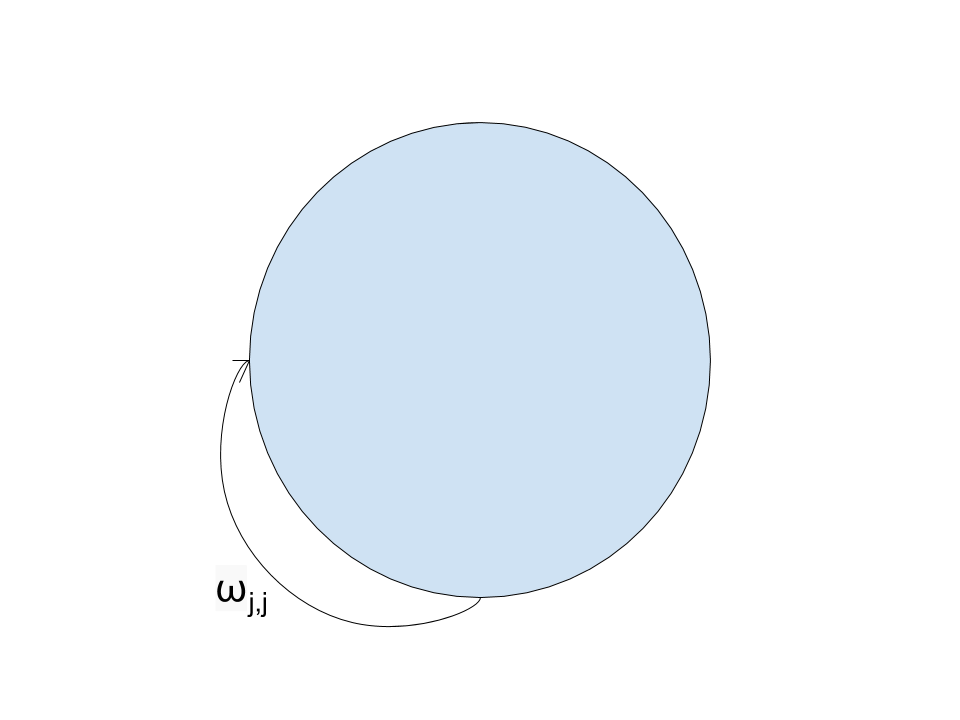
\includegraphics[width=5cm]{fig/one_recurrent_neuron}
\caption{One recurrently connected neuron. This enables a type of short-term memory, potentially capturing small-scale temporal relationships in a recurrent neural network.}
\label{fig:one_recurrent_neuron}
\end{figure}

\begin{figure}
\centering
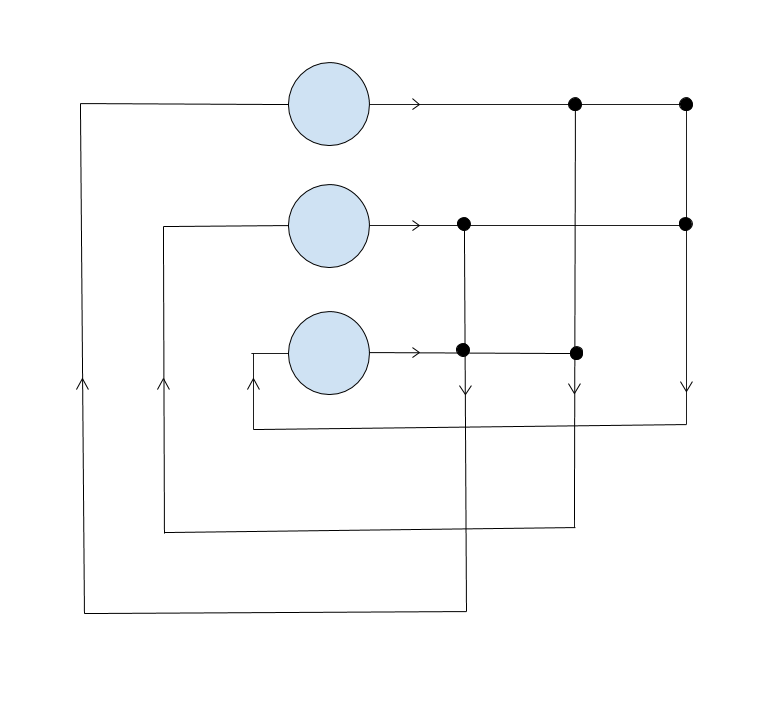
\includegraphics[width=10cm]{fig/hopfield_net}
\caption{Illustrating a simple Hopfield network - a recurrently connected neural network, consisting of three neurons. Activation values flow through the synapses back to all other neurons. This way a neuron may learn its part of a pattern, resulting in partial pattern completion if all other nodes are correctly set. Furthermore, if few patterns relative to the number of neurons are learned, the pattern completion will be more robust, requiring less  information for pattern completion. Note that transfer functions are necessary in this type of network if activation values are propagated without reduction through all synapses.}
\label{fig:hopfield_net}
\end{figure}

% ====================================
\subsection{Training RNNs}

As one might guess, a fully connected RNN may exhibit cyclic firing patterns, thus constituting a steady-state. This type of dynamics complicates the learning process, making gradient descent as elaborated on in section \ref{BP} a poor candidate for both fully connected recurrent networks, as well as other types of recurrent networks. \cite{Bengio2013b} explains that while gradient-based optimization such as gradient descent may be used to train RNNs, it generally fails to capture temporal dependencies, especially long-term dependencies. One way of alleviating the problem is by having the recurrent units of an RNN change more slowly, lowering the likelihood for an explosive gradient in certain areas. See section \ref{GRU} (GRUs) for methods that have been successful in capturing long-term dependencies in RNNs and deep learning.

% ====================================
\subsection{The Gated Recurrent Unit}\label{GRU}

\cite{Cho2014} proposed a novel ANN unit for statistical machine translation using the auto-encoder approach for two RNNs. In their paper the unit was only termed a hidden unit, but as it has later been termed the gated recurrent unit (GRU), this is what we will refer to the unit as throughout this thesis. The GRU is largely inspired by the LSTM, and appears to implement the same behaviour as the LSTM. Therefore we have only chosen to include the formal background for the GRU. As proposed by \cite{Cho2014}, the GRU may be formally defined as follows,

\begin{equation}
    r_j = \sigma ([\textbf{W}_r \textbf{x}]_j + [\textbf{U}_r\textbf{h}_{<t-1>}]_j), 
\end{equation}
where $\sigma$ is the sigmoid function, $\textbf{W}$ are the weights for the input layer $\textbf{x}$, and $\textbf{U}$ are the input weights for the hidden layer $\textbf{h}$.

Furthermore, \cite{Cho2014} defines the update gate $z_j$ as,

\begin{equation}
    z_j = \sigma([\textbf{W}_z\textbf{x}]_j + [\textbf{U}\textbf{h}_{<t-1>}]_j)
\end{equation}
 
With the activation of a hidden state $h_j$ as,
 
\begin{equation}
    h_j^{<t>} = z_j h_j^{<t-1>} + (1 - z_j) \tilde{h}_j^{<t>},
\end{equation}
 
defining,
 
\begin{equation}
    \tilde{h}_j^{<t>} = \phi ([\textbf{W}\textbf{x}]_j + [\textbf{U}(\textbf{r} \odot \textbf{h}_{<t-1>})]_j)
\end{equation}

\begin{figure}
\centering
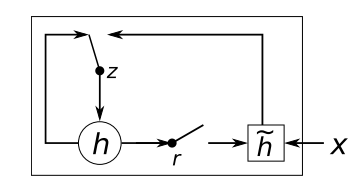
\includegraphics{fig/cho_gru}
\caption{\cite{Cho2014} illustrates their proposed hidden unit, later termed the gated recurrent unit. As outlined in the euqations of \cite{Cho2014} above, the GRU determines whether a hidden state should be updated, and ignored through $z$, and $r$, respectively.}
\label{fig:cho_gru}
\end{figure}

The formulae proposed by \cite{Cho2014}, here presented above, effectively lets an RNN capture long-term temporal dependencies through the correct parametrization of the proposed GRU. Furthermore, a gradient-based approach may be used to estimate the model weights (\cite{Cho2014}).


% ====================================
\subsection{Multiple-timescales recurrent neural networks}

\cite{Tani2014} investigates the emergence of a functional hierarchy of motor primitives in a multiple-timescales recurrent neural network (MTRNN). It consists of two continuous timescale recurrent neural networks (CTRNNs) as sub-networks, operating at two different timescales. See figure \ref{fig:tani_2014_mtrnn} for an illustration of the structure which \cite{Tani2014} proposes.

\begin{figure}
\centering
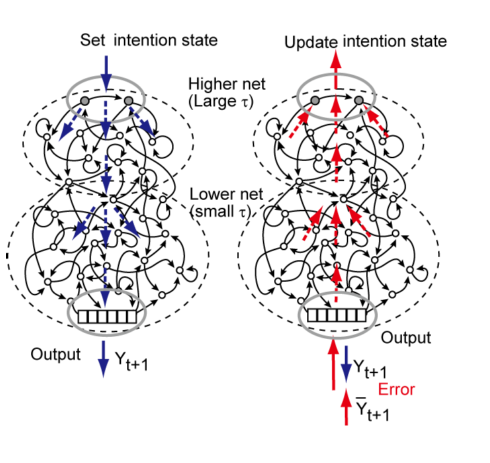
\includegraphics[width=8cm]{fig/tani_2014_mtrnn}
\caption{An illustration by \cite{Tani2014}, in which he illustrates the FFBP process in the proposed MTRNN.}
\label{fig:tani_2014_mtrnn}
\end{figure}

Formally, \cite{Tani2014} proposes the following neural dynamics,

\begin{equation}\label{tani_membrane_potential}
    \tau_i\dot{u}_i = -u_i + \sum_{j}{}\omega_{i,j}a_j + \sum_{k}{}\omega_{i,k} I_k,
\end{equation}

where $\tau_i$ is the time constant, $u_i$ is the membrane potential, $a_i$ is the neural activation state for an internal unit, $y_i$ is the neural activation state for an output unit, and $b_i$ is a bias unit, the subscript denoting a neuron $i$. $\dot{u}_i = \frac{d}{d t}u_i$.

Internal neurons use a sigmoidal transfer function with the sum of the activation and bias values, 

\begin{center}\begin{math}
    a_i = \frac{1}{1+e^{-(u_i+b_i)}},
\end{math}\end{center}
whereas the output neurons use a softmax function,

\begin{equation}\label{tani_softmax}
    y_i = \frac{e^{u_i}}{\sum_{j \in Out}^{}{e^{u_j}}},
\end{equation}
Note that this leads to a fairly sparse representation, where $\sum_{i=1}^{K} y_i = 1$.

In order to train an MTRNN, \cite{Tani2014} defines the Kullback-Leibler divergence as the error criteria $E$ which is to be minimized in order to obtain gradients for weight updates. He then proceeds to derive a formula for recursively calculating $\frac{\partial E}{\partial u_{i,t}}$, which is very similar to a discrete time version of BPTT, and shows that it in fact becomes the discrete BPTT for a certain parameter setting ($\tau=1$). The resulting equations are as follows:

\begin{equation}\label{Kullback_Leibler_divergence}
    E = \sum_t \sum_{i \in Out} y_{i,t}^* log(\frac{y_{i,t}^*}{y_{i,t}}),
\end{equation}
where $y_{i,t}^*$ is the target output and $y_{i,t}$ is the current output for neuron $i$ at time $t$.

\begin{equation}
    \omega_{i,j}(n+1) = \omega_{i,j}(n) - \alpha\frac{\partial E}{\partial \omega_{i,j}},
\end{equation}
where $n$ is the $n$-th iteration step during learning.

\begin{equation}
    \frac{\partial E}{\partial \omega_{i,j}} = \sum_{t} \frac{1}{\tau_i}\frac{\partial E}{\partial u_{i,t}a_{j,t-1}},
\end{equation}
where

\begin{equation}
    \frac{\partial E}{\partial u_{i,t}} = \begin{cases}
        y_{i,t} - y_{i,t}^* + (1-\frac{1}{\tau_i} \frac{\partial E}{\partial u_{i,t+1}}), \text{if $i \in Out$} \\
        \sum_{k \in N}\frac{\partial E}{\partial u_{k,t+1}}[\delta_{i,k}(1-\frac{1}{\tau_i})+\frac{1}{\tau_k}\omega_{k,i}f'(u_{i,t})], \text{if $\notin Out$}
   \end{cases}
\end{equation}
where $\delta$ is the Kronecker Delta function, i.e.,

\begin{center}
\begin{math}
    \delta = \begin{cases}
        0, \text{if $i \neq k$} \\
        1, \text{if $i = k$}
    \end{cases}
\end{math}
\end{center}

The MTRNN improves the PB-vector approach, where the synchronization of two modules that extract the 'knowledge' to perform two distinct tasks occurs. We find this very interesting (and intriguing) in terms of the self-organization of a functional hierarchy, and we wish to investigate the possible applications of this approach in the dual-network memory architecture. Namely whether an MTRNN could be used in extracting a functional hierarchy to and from the neocortical network. This could have potential implications for re-instantiation of previously learned functionality from the neocortical network into the hippocampal network. Another aspect that is worth emphasizing is that it could possibly enable the neocortical network to organize its memories in a more meaningful way.


\section{Summary}

Because GRUs enable an RNN to remember long-term temporal dependencies, we propose that it may improve the quality of interleaved memories in the dual-network memory architecture. More specifically, by attaining a more robust long-term memory for the learned patterns. Furthermore, we wish to investigate whether this may also enable the neocortical module to learn more elaborate patterns and functions, i.e. that capturing temporal long-term dependencies may enhance the networks internal representations in the dual-network memory architecture.
Another aspect we wish to further investigate in our future work is the ability of the hippocampal module to determine stability in pattern abstraction. As the hippocampal network exhibits a form of deterministic chaos, i.e. very long cycles appearing as chaos, or cycles that may be observed to be basins of attraction, a convergence criteria for stability may be formulated. More specifically, this could possibly be done by regarding the convergence of the HPC module for a given stream of input with learning. If the patterns appear stable, they could be consolidated to a neocortical network, similar to what is done by \cite{Hattori2014}. Analogously, we wish to investigate possible implications for determining the stability of abstraction, with the aim of gaining further insight into possible mechanisms for abstraction across memories in ANN models. This may have implications within the domain of unsupervised learning, deep learning, neuroscience, and psychology.

\section{Notes}

I should include a section with algorithmic implications, i.e. that the gradient-based approach may be performed 'decentralized' a.k.a. highly parallelized because the gradients of the former time-steps may be used in the chain-rule, yet resulting in stability and convergence towards a solution. Need to find a source on this. Didn't I read a paper stating that this could be shown? Should consult its details..


\cleardoublepage